\chapter{Deriving other gates from universal gates}
%\ref{sec:background}.

\section{Aim}
%\label{sec:objectives}
	To implement the logic functions i.e. AND, OR, NOT, Ex-OR, Ex- NOR and a logical expression with the help of NAND and NOR universal gates respectively.

\section{Apparatus}
%\label{sec:objectives}
	\begin{itemize}
		\tightlist
		\item Kit for realization of NAND and NOR gates
		\item Connecting Leads
	\end{itemize}

\section{Theory}
	Logic gates are electronic circuits which perform logical functions on one or more inputs to produce one output. There are seven logic gates. When all the input combinations of a logic gate are written in a series and their corrresponding outputs written along them, then this input/ output combination is called Truth Table.
	
	AND, OR, NOT, XOR and XNOR gates can be derived from NAND and NOR gates by converting their respective equations to NAND or NOR form, using he following 3 laws of Boolean Algebra (and their duals according to Duality Principle):
	\begin{enumerate}
		\tightlist
		\item Involution Law: $\overline{(\overline{X})} = X$
		\item Idempotent Law: $X + X = X$
		\item De-Morgan's Law: $\overline{X+Y} = \overline{X} . \overline{Y}$
	\end{enumerate}
	
	\subsection{NAND gate}
		NAND gate is actually a combination of two logic gates i.e. AND gate followed by NOT gate. So its output is complement of the output of an AND gate.This gate can have minimum two inputs. By using only NAND gates, we can realize all logic functions: AND, OR, NOT, Ex-OR, Ex-NOR, NOR. So this gate is also called as universal gate.
		The expression for NAND gate is:
		$$Y = \overline{A.B}$$
	\subsection{NOR gate}
		NOR gate is actually a combination of two logic gates: OR gate followed by NOT gate. So its output is complement of the output of an OR gate.This gate can have minimum two inputs, output is always one. By using only NOR gates, we can realize all logic functions: AND, OR, NOT, Ex-OR, Ex-NOR, NAND. So this gate is also called universal gate.
		The expression for NOR gate is:
		$$Y = \overline{A+B}$$

\section{Circuits}
	\subsection{NAND gate as Universal gate}
		\subsubsection{NAND gates as OR gate}			
			From DeMorgan’s theorems:
			\begin{align*}
				(A.B)^\prime &= A^\prime + B^\prime \\
				(A^\prime .B^\prime)^\prime &= A^{\prime\prime} + B^{\prime\prime} \\
				&= A + B
			\end{align*}
			So, give the inverted inputs to a NAND gate, obtain OR operation at output.
			\begin{figure}[ht]
				\centering
				\subfloat[OR gate using NAND gates]{
					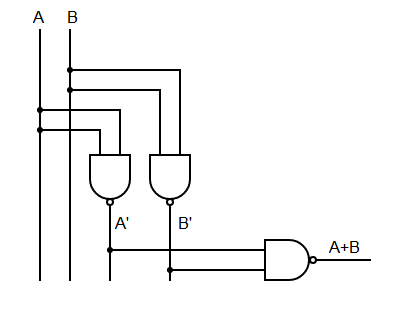
\includegraphics[width=0.6\textwidth,valign=c]{img/exp4/fig1}
					\label{fig:nand_to_or:1}
				}
				\hfill
				\subfloat[Truth Table for OR]
				{
					\begin{tabular}{|c|c|c|}
						\hline
						\multicolumn{2}{|c|}{Input} & Output \\
						\hline
						$A$ & $B$ & $Y=A + B$ \\
						\hline
						0 & 0 & 0 \\
						\hline
						0 & 1 & 1 \\
						\hline
						1 & 0 & 1 \\
						\hline
						1 & 1 & 1 \\
						\hline
					\end{tabular}
					\label{fig:nand_to_or:2}
				}
				\caption{\textit{OR Gate}}
			\end{figure}			
	
		\subsubsection{NAND gates as AND gate}
			From DeMorgan’s theorems:
			\begin{align*}
				Y &= ((A.B)^\prime)^\prime \\
				Y &= (A.B)				
			\end{align*}
			A NAND produces complement of AND gate. So, if the output of a NAND gate is inverted, overall output will be that of an AND gate.
			\begin{figure}[ht]
				\centering
				\subfloat[AND gate using NAND gates]{
					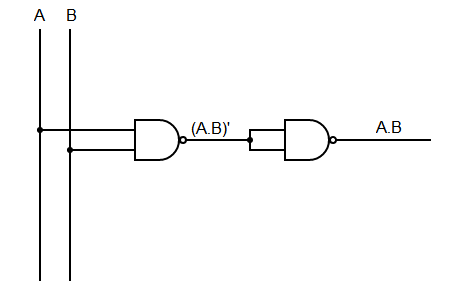
\includegraphics[width=0.6\textwidth,valign=c]{img/exp4/fig2}
					\label{fig:nand_to_and:1}
				}
				\hfill
				\subfloat[Truth Table for AND]
				{
					\begin{tabular}{|c|c|c|}
						\hline
						\multicolumn{2}{|c|}{Input} & Output \\
						\hline
						$A$ & $B$ & $Y=A . B$ \\
						\hline
						0 & 0 & 0 \\
						\hline
						0 & 1 & 0 \\
						\hline
						1 & 0 & 0 \\
						\hline
						1 & 1 & 1 \\
						\hline
					\end{tabular}
					\label{fig:nand_to_and:2}
				}
				\caption{\textit{AND Gate}}
			\end{figure}
			
		\subsubsection{NAND gates as XOR gate}
			From DeMorgan’s theorems:
			\begin{align*}
				Y &= A \oplus B \\
				  &= \overline{A}B + A\overline{B} \\
				  &= \overline{(\overline{\overline{A}B + A\overline{B}})} \\
				  &= \overline{(\overline{(\overline{A}B)} . \overline{(A\overline{B})})} \\
				  &= \overline{(A+\overline{B}) . (\overline{A} + B)}
			\end{align*}
			This can be achieved with the logic diagram shown in Figure \ref{fig:nand_to_xor:1}.
			\begin{figure}[ht]
				\centering
				\subfloat[XOR gate using NAND gates]{
					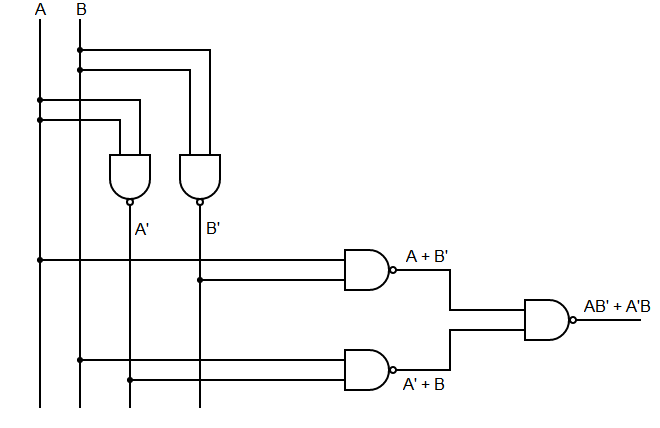
\includegraphics[width=0.6\textwidth,valign=c]{img/exp4/fig3}
					\label{fig:nand_to_xor:1}
				}
				\hfill
				\subfloat[Truth Table for XOR]
				{
					\begin{tabular}{|c|c|c|}
						\hline
						\multicolumn{2}{|c|}{Input} & Output \\
						\hline
						$A$ & $B$ & $Y=A \oplus B$ \\
						\hline
						0 & 0 & 0 \\
						\hline
						0 & 1 & 1 \\
						\hline
						1 & 0 & 1 \\
						\hline
						1 & 1 & 0 \\
						\hline
					\end{tabular}
					\label{fig:nand_to_xor:2}
				}
				\caption{\textit{XOR Gate}}
			\end{figure}
		
		\subsubsection{NAND gates as XNOR gate}
			From DeMorgan’s theorems:
			\begin{align*}
				Y &= \overline{A \oplus B} \\
				&= \overline{(\overline{A}B + A\overline{B})} \\
				&= \overline{(\overline{(\overline{\overline{A}B + A\overline{B}})})} \\
				&= \overline{(\overline{(\overline{(\overline{A}B)} . \overline{(A\overline{B})})})} \\
				&= \overline{(\overline{(A+\overline{B}) . (\overline{A} + B)})} \\
				&= \overline{(XOR-gate-implemented-using-NAND-Gates)}
			\end{align*}
			The output of a two input XNOR gate is shown by: $Y = \overline{\overline{A}B + A\overline{B}}$. This can be achieved with the logic diagram shown in Figure \ref{fig:nand_to_xnor:1}.
			\begin{figure}[ht]
				\centering
				\subfloat[XNOR gate using NAND gates]{
					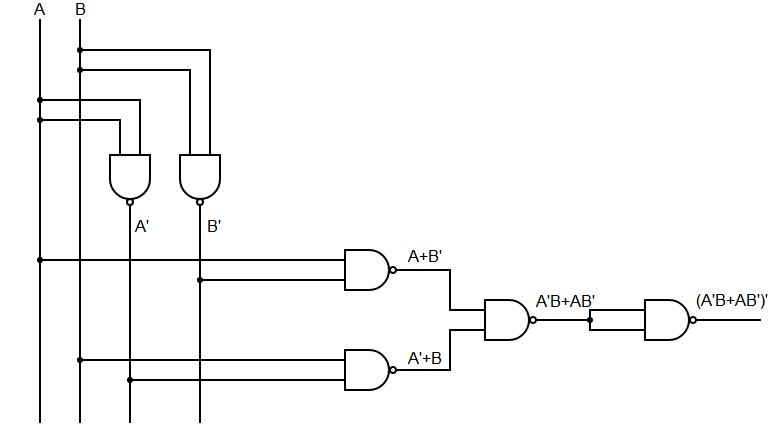
\includegraphics[width=0.6\textwidth,valign=c]{img/exp4/fig4}
					\label{fig:nand_to_xnor:1}
				}
				\hfill
				\subfloat[Truth Table for XNOR]
				{
					\begin{tabular}{|c|c|c|}
						\hline
						\multicolumn{2}{|c|}{Input} & Output \\
						\hline
						$A$ & $B$ & $Y=\overline{A \oplus B}$ \\
						\hline
						0 & 0 & 1 \\
						\hline
						0 & 1 & 0 \\
						\hline
						1 & 0 & 0 \\
						\hline
						1 & 1 & 1 \\
						\hline
					\end{tabular}
					\label{fig:nand_to_xnor:2}
				}
				\caption{\textit{XNOR Gate}}
			\end{figure}
	
	\subsection{NOR gate as Universal gate}
		\subsubsection{NOR gates as OR gate}			
		From DeMorgan’s theorems:
		\begin{align*}
			Y &= \overline{(\overline{(A+B)})} \\
			  &= (A + B)
		\end{align*}
		A NOR produces complement of OR gate. So, if the output of a NOR gate is inverted, overall output will be that of an OR gate.
		\begin{figure}[ht]
			\centering
			\subfloat[OR gate using NOR gates]{
				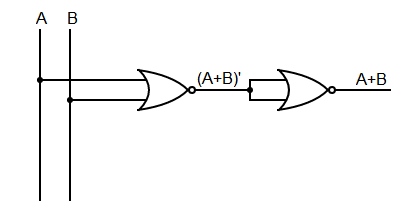
\includegraphics[width=0.6\textwidth,valign=c]{img/exp4/fig5}
				\label{fig:nor_to_or:1}
			}
			\hfill
			\subfloat[Truth Table for OR]
			{
				\begin{tabular}{|c|c|c|}
					\hline
					\multicolumn{2}{|c|}{Input} & Output \\
					\hline
					$A$ & $B$ & $Y=A + B$ \\
					\hline
					0 & 0 & 0 \\
					\hline
					0 & 1 & 1 \\
					\hline
					1 & 0 & 1 \\
					\hline
					1 & 1 & 1 \\
					\hline
				\end{tabular}
				\label{fig:nor_to_or:2}
			}
			\caption{\textit{OR Gate}}
		\end{figure}			
		
		\subsubsection{NOR gates as AND gate}
		From DeMorgan’s theorems:
		\begin{align*}
			Y &= A.B \\
			  &= \overline{(\overline{A.B})} \\
			  &= \overline{(\overline{A} + \overline{B})}
		\end{align*}
		So, give the inverted inputs to a NOR gate, obtain AND operation at output.
		\begin{figure}[ht]
			\centering
			\subfloat[AND gate using NAND gates]{
				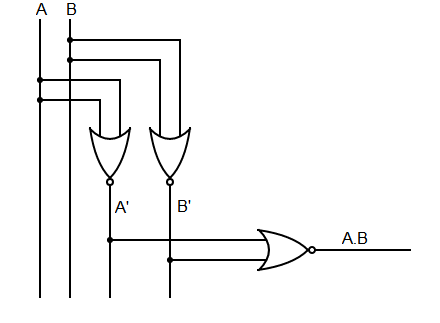
\includegraphics[width=0.6\textwidth,valign=c]{img/exp4/fig6}
				\label{fig:nor_to_and:1}
			}
			\hfill
			\subfloat[Truth Table for AND]
			{
				\begin{tabular}{|c|c|c|}
					\hline
					\multicolumn{2}{|c|}{Input} & Output \\
					\hline
					$A$ & $B$ & $Y=A . B$ \\
					\hline
					0 & 0 & 0 \\
					\hline
					0 & 1 & 0 \\
					\hline
					1 & 0 & 0 \\
					\hline
					1 & 1 & 1 \\
					\hline
				\end{tabular}
				\label{fig:nor_to_and:2}
			}
			\caption{\textit{AND Gate}}
		\end{figure}
		
		\subsubsection{NOR gates as XOR gate}
		From DeMorgan’s theorems:
		\begin{align*}
			Y &= A \oplus B \\
			&= \overline{A}B + A\overline{B} \\
			&= \overline{(\overline{\overline{A}B + A\overline{B}})} \\
			&= \overline{(\overline{(\overline{A}B)} . \overline{(A\overline{B})})} \\
			&= \overline{(A+\overline{B}) . (\overline{A} + B)} \\
			&= \overline{(A+\overline{B})} + \overline{(\overline{A} + B)} \\
			&= M + N \\
			&= \overline{(\overline{M+N})} \\
			\\
			M = \overline{(A+\overline{B})} &, N = \overline{(\overline{A} + B)}
		\end{align*}
		The output of a two input Ex-OR gate is shown by: $Y = \overline{A}B + A\overline{B}$. This can be achieved with the logic diagram shown in Figure \ref{fig:nor_to_xor:1}.
		\begin{figure}[ht]
			\centering
			\subfloat[XOR gate using NOR gates]{
				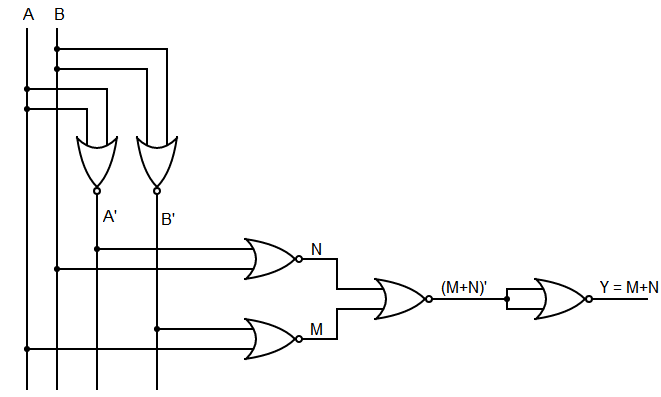
\includegraphics[width=0.6\textwidth,valign=c]{img/exp4/fig7}
				\label{fig:nor_to_xor:1}
			}
			\hfill
			\subfloat[Truth Table for XOR]
			{
				\begin{tabular}{|c|c|c|}
					\hline
					\multicolumn{2}{|c|}{Input} & Output \\
					\hline
					$A$ & $B$ & $Y=A \oplus B$ \\
					\hline
					0 & 0 & 0 \\
					\hline
					0 & 1 & 1 \\
					\hline
					1 & 0 & 1 \\
					\hline
					1 & 1 & 0 \\
					\hline
				\end{tabular}
				\label{fig:nor_to_xor:2}
			}
			\caption{\textit{XOR Gate}}
		\end{figure}
		
		\subsubsection{NOR gates as XNOR gate}
		From DeMorgan’s theorems:
		\begin{align*}
			Y &= \overline{A \oplus B} \\
			&= \overline{\overline{A}B + A\overline{B}} \\
			&= \overline{\overline{(\overline{\overline{A}B + A\overline{B}})}} \\
			&= \overline{\overline{(\overline{(\overline{A}B)} . \overline{(A\overline{B})})}} \\
			&= \overline{\overline{(A+\overline{B}) . (\overline{A} + B)}} \\
			&= \overline{\overline{(A+\overline{B})} + \overline{(\overline{A} + B)}} \\
			&= \overline{M + N} \\
			\\
			M = \overline{(A+\overline{B})} &, N = \overline{(\overline{A} + B)}
		\end{align*}
		The output of a two input Ex-NOR gate is shown by: $Y = \overline{\overline{A}B + A\overline{B}}$. This can be achieved with the logic diagram shown in Figure \ref{fig:nor_to_xnor:1}.
		\begin{figure}[ht]
			\centering
			\subfloat[XNOR gate using NOR gates]{
				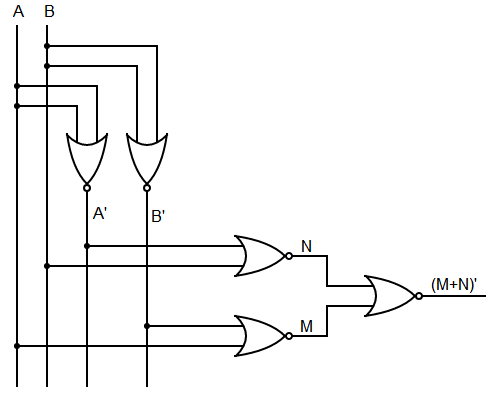
\includegraphics[width=0.6\textwidth,valign=c]{img/exp4/fig8}
				\label{fig:nor_to_xnor:1}
			}
			\hfill
			\subfloat[Truth Table for XNOR]
			{
				\begin{tabular}{|c|c|c|}
					\hline
					\multicolumn{2}{|c|}{Input} & Output \\
					\hline
					$A$ & $B$ & $Y=\overline{A \oplus B}$ \\
					\hline
					0 & 0 & 1 \\
					\hline
					0 & 1 & 0 \\
					\hline
					1 & 0 & 0 \\
					\hline
					1 & 1 & 1 \\
					\hline
				\end{tabular}
				\label{fig:nor_to_xnor:2}
			}
			\caption{\textit{XOR Gate}}
		\end{figure}

\section{Procedure}
	\begin{enumerate}
		\tightlist
		\item Check the components for their working (NAND or NOR kit).
		\item Insert the wire-leads into the appropriate places on the kit as per the cicuits shown.
		\item For output, use the LED on the provided kit.
		\item Provide the input data in the input switches and observe the output on the LED.
		\item Verify the truth tables of various gates.
	\end{enumerate}

\section{Precautions}
	\begin{enumerate}
		\tightlist
		\item The leads must be connected properly.
		\item Wires must be connected during power supply being off only.
		\item Change the input switches only when supply is off.
	\end{enumerate}

\section{Result}
	NOT, AND, OR, XOR, XNOR gates can be realized using NAND and NOR gates.